%--------------------------------------------------------------------
% NE 155 (intro to numerical simulation of radiation transport)
% Spring 2014

% formatting
\documentclass[12pt]{article}
\usepackage[top=1in, bottom=1in, left=1in, right=1in]{geometry}

\usepackage{setspace}
\onehalfspacing

\setlength{\parindent}{0mm} \setlength{\parskip}{1em}


% packages
\usepackage{amssymb}
%% The amsthm package provides extended theorem environments
\usepackage{amsthm}
\usepackage{epsfig}
\usepackage{times}
\renewcommand{\ttdefault}{cmtt}
\usepackage{amsmath}
\usepackage{graphicx} % for graphics files

% Draw figures yourself
\usepackage{tikz} 

% The float package HAS to load before hyperref
\usepackage{float} % for psuedocode formatting
\usepackage{xspace}

% from Denovo methods manual
\usepackage{mathrsfs}
\usepackage[mathcal]{euscript}
\usepackage{color}
\usepackage{array}

\usepackage[pdftex]{hyperref}

\newcommand{\nth}{n\ensuremath{^{\text{th}}} }
\newcommand{\ve}[1]{\ensuremath{\mathbf{#1}}}
\newcommand{\macro}{\ensuremath{\Sigma}}
\newcommand{\vOmega}{\ensuremath{\hat{\Omega}}}

\newcommand{\cc}[1]{\ensuremath{\overline{#1}}}
\newcommand{\ccm}[1]{\ensuremath{\overline{\mathbf{#1}}}}


%--------------------------------------------------------------------
%--------------------------------------------------------------------
\begin{document}
\begin{center}
{\bf NE 155, Classes 11 \& 12, S14 \\
Approximation and Interpolation \\ February 14 and 19, 2014}
\end{center}

\setlength{\unitlength}{1in}
\begin{picture}(6,.1) 
\put(0,0) {\line(1,0){6.25}}         
\end{picture}

%--------------------------------------------------------------------
Sometimes rather than calculating values of a function, we need to approximate them instead. Why might we do this?
%
\begin{itemize}
\item It may be difficult or impossible to analytically evaluate the function
\item We may have only a table of values at certain points and need to
determine the values in between
\item It may be much faster to compute values of an approximation
function than of the original function, particularly if we have to
calculate the function values over and over again
\item A function may be defined implicitly
\end{itemize}

\textbf{Approximation}
The approximation function does \underline{not}
need to fit through all given function values

\textbf{Interpolation}
The interpolation function does need to do
through all give values of the function.


%--------------------------------------------------------------------
%--------------------------------------------------------------------
\section{Types}
Usually, an approximating function is a linear combination of
simpler functions:
%
\begin{itemize}
\item $f(x)$: function to be approximated
\item $g(x)$: approximating function = $\sum_i a_i Ci(x)$
\end{itemize}
%
Examples
%
\begin{itemize}
\item \textbf{Polynomial}: $g(x) = P(x) = \sum_i a_i x^i$

\item \textbf{Piecewise polynomial}: slap some polynomials together so their ends meet

\item \textbf{Fourier series}: $g(x) = \frac{1}{2} a_0 + \sum_i [a_i \sin(ix) + b_i \cos(ix)]$ %http://mathworld.wolfram.com/FourierSeries.html

\item Combination of \textbf{rational functions}: $g(x) = R_n(x)/R_m(x)$

\item \textbf{Exponential functions}: $g(x) = \sum_i a_i \exp(b_i x^i)$
\end{itemize}


%--------------------------------------------------------------------
%--------------------------------------------------------------------
\section{Taylor Polynomial}
If $f(x)$ is known but difficult to evaluate, we can replace it by the
Taylor polynomial around x = a
\begin{align}
f(x) &= f(a) + f'(a)(a-x) + f''(a)\frac{(x-a)^2}{2!} + \cdots + f^{(n-1)}(a)\frac{(x-a)^{n-1}}{(n-1)!} + R_n \\
%
  &= \sum_{k=0}^{n-1}\frac{(x-a)^k}{k!}f^{(k)}(a) + R_n \\
%
R_n &= f^{(n)}(x^*)\frac{(x-a)^{n}}{n!} \qquad \text{for some } x^* \in [a, x]
%http://mathworld.wolfram.com/TaylorSeries.html
\end{align}

Show Picture when you transition to Lagrange demo.

%\begin{figure}[h!]
%\begin{center}
%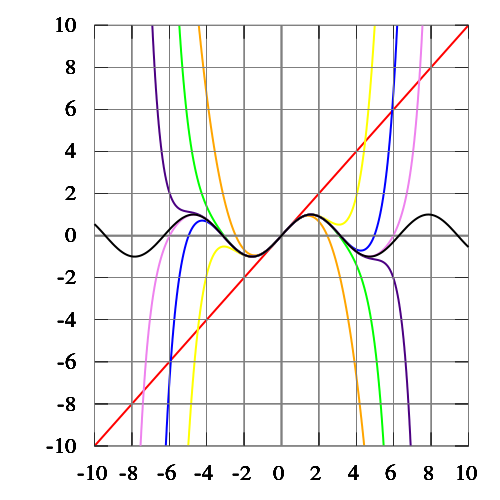
\includegraphics[height=3in,clip]{TaylorSinEg}
%\caption{As the degree of the Taylor polynomial rises, it approaches the correct function. This image shows $\sin(x)$ and its Taylor approximations, polynomials of degree 1, 3, 5, 7, 9, 11 and 13.}
%\end{center}
%\end{figure}


%--------------------------------------------------------------------
%--------------------------------------------------------------------
\section{Lagrange Interpolating Polynomial}
If $x_0, x_1,\dots, x_n$ are $(n+1)$ distinct numbers and $f(x)$ is a function defined by these numbers, then there exists a unique polynomial $P(x)$ of degree at most $n$ with the property
%
\begin{align}
f(x_k) &= P(x_k)\:, \qquad \text{for }k= 0, 1, \dots, n \\
%
P(x) &= f(x_0)L_0(x) + \dots + f(x_n)L_n(x) = \sum_{k=0}^{n}f(x_k)L_k(x) \\
%
L_k(x) &= \prod_{i=0, i \neq k}^n \frac{(x-x_i)}{(x_k-x_i)}\\
%
L_k(x) &= \frac{(x-x_0)(x-x_1)\cdots(x-x_{k-1})(x-x_{k+1})\cdots(x-x_n)}{(x_k-x_0)(x_k-x_1)\cdots(x_k-x_{k-1})(x_k-x_{k+1})\cdots(x_k-x_n)}
\end{align}

%--------------------------------------------------------------------
\section{Error}
If $f$ is $n+1$ times continuously differentiable on a closed interval $I$

and $P_{n}(x)$ is a polynomial (any polynomial) of degree at most $n$ that interpolates $f$ at $n + 1$ distinct points ${x_i}, (i=0,1,\dots,n)$ in that interval,

then for each $x$ in the interval there exists $\xi$  in that interval such that
%http://en.wikipedia.org/wiki/Polynomial_interpolation
\begin{align}
f(x) - P_n(x)& = \frac{f^{n+1}(\xi)}{(n+1)!}(x-x_0)(x-x_1)\cdots(x-x_n) \\
&\boxed{e = \frac{f^{n+1}(\xi)}{(n+1)!}\prod_{i=0}^n (x-x_i)}
\end{align}

The Lagrange polynomial of degree $n$ uses information at the
distinct numbers $x_0, x_1,\dots, x_n$ and, in place of $(x-x_0)^n$, its error formula uses a product of the $n+1$ terms.

\textbf{iPython demo; show Taylor picture as well.}

For all polynomial interpolations, the error is related to the $n+1$st derivative of the function. If we have more points than derivatives, this might not work well. This is related to our next idea.


%--------------------------------------------------------------------
%--------------------------------------------------------------------
\section{Piecewise Polynomials}

It is often difficult to get one polynomial to fit all of our data very well. 

High-degree polynomial functions have an oscillatory nature, and often a fluctuation over a small portion of the interval can induce large fluctuations and restrict their use.

This is especially true at the endpoints (you can see that from our Lagrange example).

An alternative approach is to divide the interval into small sub-intervals (usually of equal size) and construct a polynomial on each-subinterval.

The simplest way to do this is \textbf{piecewise linear}. What might be a problem with that?

If you think about our error analysis, we'd like 
\begin{enumerate}
\item to be able to differentiate our function to a degree that allows us to do error analysis give our polynomial.

Thus, we use lower order polynomials all stuck together.

\item our polynomials to be as continuously differentiable at the boundaries as possible.

Thus, we often select splines. 
\end{enumerate}
%
A \textbf{spline} is a polynomial function that is piecewise-defined, and possesses a high degree of smoothness at the places where the polynomial pieces connect (which are known as \textit{knots}).

The most common approach is to use cubic splines between each successive pair of nodes. For cubic splines, we can get continuous 2nd derivatives at the knots - which is all we can ask from cubic polynomials. 



%--------------------------------------------------------------------
%--------------------------------------------------------------------
%\bibliographystyle{plain}
%\bibliography{LinearSolns} 

\end{document}